% ******************************* PhD Thesis Template **************************
% Please have a look at the README.md file for info on how to use the template

\documentclass[a4paper,12pt,times,numbered,print,index]{Classes/PhDThesisPSnPDF}

% ******************************************************************************
% ******************************* Class Options ********************************
% *********************** See README for more details **************************
% ******************************************************************************

% `a4paper'(The University of Cambridge PhD thesis guidelines recommends a page
% size a4 - default option) or `a5paper': A5 Paper size is also allowed as per
% the Cambridge University Engineering Deparment guidelines for PhD thesis
%
% `11pt' or `12pt'(default): Font Size 10pt is NOT recommended by the University
% guidelines
%
% `oneside' or `twoside'(default): Printing double side (twoside) or single
% side.
%
% `print': Use `print' for print version with appropriate margins and page
% layout. Leaving the options field blank will activate Online version.
%
% `index': For index at the end of the thesis
%
% `draftclassic': For draft mode without loading any images (same as draft in book)
%
% `draft': Special draft mode with line numbers, images, and water mark with
% timestamp and custom text. Position of the text can also be modified.
%
% `abstract': To generate only the title page and abstract page with
% dissertation title and name, to submit to the Student Registry
%
% `chapter`: This option enables only the specified chapter and it's references
%  Useful for review and corrections.
%
% ************************* Custom Page Margins ********************************
%
% `custommargin`: Use `custommargin' in options to activate custom page margins,
% which can be defined in the preamble.tex. Custom margin will override
% print/online margin setup.
%
% *********************** Choosing the Fonts in Class Options ******************
%
% `times' : Times font with math support. (The Cambridge University guidelines
% recommend using times)
%
% `fourier': Utopia Font with Fourier Math font (Font has to be installed)
%            It's a free font.
%
% `customfont': Use `customfont' option in the document class and load the
% package in the preamble.tex
%
% default or leave empty: `Latin Modern' font will be loaded.
%
% ********************** Choosing the Bibliography style ***********************
%
% `authoryear': For author-year citation eg., Krishna (2013)
%
% `numbered': (Default Option) For numbered and sorted citation e.g., [1,5,2]
%
% `custombib': Define your own bibliography style in the `preamble.tex' file.
%              `\RequirePackage[square, sort, numbers, authoryear]{natbib}'.
%              This can be also used to load biblatex instead of natbib
%              (See Preamble)
%
% **************************** Choosing the Page Style *************************
%
% `default (leave empty)': For Page Numbers in Header (Left Even, Right Odd) and
% Chapter Name in Header (Right Even) and Section Name (Left Odd). Blank Footer.
%
% `PageStyleI': Chapter Name next & Page Number on Even Side (Left Even).
% Section Name & Page Number in Header on Odd Side (Right Odd). Footer is empty.
%
% `PageStyleII': Chapter Name on Even Side (Left Even) in Header. Section Number
% and Section Name in Header on Odd Side (Right Odd). Page numbering in footer

% Uncomment to change page style
%\pagestyle{PageStyleII}

% ********************************** Preamble **********************************
% Preamble: Contains packages and user-defined commands and settings
% ******************************************************************************
% ****************************** Custom Margin *********************************

% Add `custommargin' in the document class options to use this section
% Set {innerside margin / outerside margin / topmargin / bottom margin}  and
% other page dimensions
\ifsetCustomMargin
  \RequirePackage[left=37mm,right=30mm,top=35mm,bottom=30mm]{geometry}
  \setFancyHdr % To apply fancy header after geometry package is loaded
\fi

% Add spaces between paragraphs
%\setlength{\parskip}{0.5em}
% Ragged bottom avoids extra whitespaces between paragraphs
\raggedbottom
% To remove the excess top spacing for enumeration, list and description
%\usepackage{enumitem}
%\setlist[enumerate,itemize,description]{topsep=0em}

% *****************************************************************************
% ******************* Fonts (like different typewriter fonts etc.)*************

% Add `customfont' in the document class option to use this section

\ifsetCustomFont
  % Set your custom font here and use `customfont' in options. Leave empty to
  % load computer modern font (default LaTeX font).
  %\RequirePackage{helvet}

  % For use with XeLaTeX
  %  \setmainfont[
  %    Path              = ./libertine/opentype/,
  %    Extension         = .otf,
  %    UprightFont = LinLibertine_R,
  %    BoldFont = LinLibertine_RZ, % Linux Libertine O Regular Semibold
  %    ItalicFont = LinLibertine_RI,
  %    BoldItalicFont = LinLibertine_RZI, % Linux Libertine O Regular Semibold Italic
  %  ]
  %  {libertine}
  %  % load font from system font
  %  \newfontfamily\libertinesystemfont{Linux Libertine O}
\fi

% *****************************************************************************
% **************************** Custom Packages ********************************
% ************************* Indent the first line after a new section **************************
\usepackage{indentfirst}

% ************************* Algorithms and Pseudocode **************************

%\usepackage{algpseudocode}

% ********************Captions and Hyperreferencing / URL **********************

% Captions: This makes captions of figures use a boldfaced small font.
%\RequirePackage[small,bf]{caption}

\RequirePackage[labelsep=space,tableposition=top]{caption}
\renewcommand{\figurename}{Fig.} %to support older versions of captions.sty


% *************************** Graphics and figures *****************************

%\usepackage{rotating}
%\usepackage{wrapfig}

% Uncomment the following two lines to force Latex to place the figure.
% Use [H] when including graphics. Note 'H' instead of 'h'
\usepackage{float}
\restylefloat{figure}

% Subcaption package is also available in the sty folder you can use that by
% uncommenting the following line
% This is for people stuck with older versions of texlive
%\usepackage{sty/caption/subcaption}
\usepackage{subcaption}

% ********************************** Tables ************************************
\usepackage{booktabs} % For professional looking tables
\usepackage{multirow}

%\usepackage{multicol}
%\usepackage{longtable}
%\usepackage{tabularx}


% *********************************** SI Units *********************************
\usepackage{siunitx} % use this package module for SI units


% ******************************* Line Spacing *********************************

% Choose linespacing as appropriate. Default is one-half line spacing as per the
% University guidelines

% \doublespacing
% \onehalfspacing
% \singlespacing


% ************************ Formatting / Footnote *******************************

% Don't break enumeration (etc.) across pages in an ugly manner (default 10000)
%\clubpenalty=500
%\widowpenalty=500

%\usepackage[perpage]{footmisc} %Range of footnote options


% *****************************************************************************
% *************************** Bibliography  and References ********************

%\usepackage{cleveref} %Referencing without need to explicitly state fig /table

% Add `custombib' in the document class option to use this section
\ifuseCustomBib
   \RequirePackage[square, sort, numbers, authoryear]{natbib} % CustomBib

% If you would like to use biblatex for your reference management, as opposed to the default `natbibpackage` pass the option `custombib` in the document class. Comment out the previous line to make sure you don't load the natbib package. Uncomment the following lines and specify the location of references.bib file

%\RequirePackage[backend=biber, style=numeric-comp, citestyle=numeric, sorting=nty, natbib=true]{biblatex}
%\bibliography{References/references} %Location of references.bib only for biblatex

\fi

% changes the default name `Bibliography` -> `References'
\renewcommand{\bibname}{References}


% ******************************************************************************
% ************************* User Defined Commands ******************************
% ******************************************************************************

% *********** To change the name of Table of Contents / LOF and LOT ************

%\renewcommand{\contentsname}{My Table of Contents}
%\renewcommand{\listfigurename}{My List of Figures}
%\renewcommand{\listtablename}{My List of Tables}


% ********************** TOC depth and numbering depth *************************

\setcounter{secnumdepth}{4}
\setcounter{tocdepth}{4}


% ******************************* Nomenclature *********************************

% To change the name of the Nomenclature section, uncomment the following line

%\renewcommand{\nomname}{Symbols}


% ********************************* Appendix ***********************************

% The default value of both \appendixtocname and \appendixpagename is `Appendices'. These names can all be changed via:

%\renewcommand{\appendixtocname}{List of appendices}
%\renewcommand{\appendixname}{Appndx}

% *********************** Configure Draft Mode **********************************

% Uncomment to disable figures in `draft'
%\setkeys{Gin}{draft=true}  % set draft to false to enable figures in `draft'

% These options are active only during the draft mode
% Default text is "Draft"
%\SetDraftText{DRAFT}

% Default Watermark location is top. Location (top/bottom)
%\SetDraftWMPosition{bottom}

% Draft Version - default is v1.0
%\SetDraftVersion{v1.1}

% Draft Text grayscale value (should be between 0-black and 1-white)
% Default value is 0.75
%\SetDraftGrayScale{0.8}


% ******************************** Todo Notes **********************************
%% Uncomment the following lines to have todonotes.

%\ifsetDraft
%	\usepackage[colorinlistoftodos]{todonotes}
%	\newcommand{\mynote}[1]{\todo[author=kks32,size=\small,inline,color=green!40]{#1}}
%\else
%	\newcommand{\mynote}[1]{}
%	\newcommand{\listoftodos}{}
%\fi

% Example todo: \mynote{Hey! I have a note}


% ************************ Thesis Information & Meta-data **********************
% Thesis title and author information, refernce file for biblatex
% ************************ Thesis Information & Meta-data **********************
%% The title of the thesis
\title{Blockchain Ethereum}
%\texorpdfstring is used for PDF metadata. Usage:
%\texorpdfstring{LaTeX_Version}{PDF Version (non-latex)} eg.,
%\texorpdfstring{$sigma$}{sigma}

%% Subtitle (Optional)
\subtitle{Smart Contracts en la base de datos distrubuída}

%% The full name of the author
\author{
  Echevarria Leandro
}

%% Department (eg. Department of Engineering, Maths, Physics)
\dept{Departamento de Sistemas}

%% University and Crest
\university{Universidad Tecnológica Nacional}
% Crest minimum should be 30mm.
\crest{
\includegraphics[width=0.2\textwidth]{University_Crest}}
%% Use this crest, if you are using the college crest
%% Crest long miminum should be 65mm
%\crest{\includegraphics[width=0.45\textwidth]{University_Crest_Long}}

%% College shield [optional] 
% Crest minimum should be 30mm.
%\collegeshield{\includegraphics[width=0.2\textwidth]{CollegeShields/Kings}}


%% Supervisor (optional)
%% for multiple supervisors, append each supervisor with the \newline command
%\supervisor{Prof. A.B. Supervisor\newline
%Prof. C.D. Supervisor}

%% Supervisor Role (optional) - Supervisor (default) or advisor
% \supervisorrole{\textbf{Supervisors: }}
%% if no title is desired:
% \supervisorrole{}

%% Supervisor line width: required to align supervisors
%\supervisorlinewidth{0.35\textwidth}

%% Advisor (optional)
%% for multiple advisors, append each advisor with the \newline command
%\advisor{Dr. A. Advisor\newline
%Dr. B. Advisor}
     
%% Advisor Role (optional) - Advisor (default) or leave empty
% \advisorrole{Advisors: }
%% if no title is required
% \advisorrole{}

%% Advisor line width: required to align supervisors
%\advisorlinewidth{0.25\textwidth}


%% You can redefine the submission text:
% Default as per the University guidelines:
% ``This dissertation is submitted for the degree of''
%\renewcommand{\submissiontext}{change the default text here if needed}

%% Full title of the Degree
\degreetitle{Técnico Superior en Sistemas Informáticos}

%% College affiliation (optional)
\college{Universidad Tecnológica Nacional}

%% Submission date
% Default is set as {\monthname[\the\month]\space\the\year}
%\degreedate{September 2014} 

%% Meta information
\subject{LaTeX} \keywords{{LaTeX} {PhD Thesis} {Blockchain} {Ethereum} {Smart Contracts} }


% ***************************** Abstract Separate ******************************
% To printout only the titlepage and the abstract with the PhD title and the
% author name for submission to the Student Registry, use the `abstract' option in
% the document class.

\ifdefineAbstract
 \pagestyle{empty}
 \includeonly{Declaration/declaration, Abstract/abstract}
\fi

% ***************************** Chapter Mode ***********************************
% The chapter mode allows user to only print particular chapters with references
% Title, Contents, Frontmatter are disabled by default
% Useful option to review a particular chapter or to send it to supervisior.
% To use choose `chapter' option in the document class

\ifdefineChapter
 \includeonly{Chapter3/chapter3}
\fi

% ******************************** Front Matter ********************************
\begin{document}

\frontmatter

\maketitle

% ******************************* Thesis Dedidcation ********************************

\begin{dedication} 

Queremos agradecer a \dots

\end{dedication}
% ******************************* Thesis Declaration ***************************

\begin{declaration}

I hereby declare that except where specific reference is made to the work of 
others, the contents of this dissertation are original and have not been 
submitted in whole or in part for consideration for any other degree or 
qualification in this, or any other university. This dissertation is my own 
work and contains nothing which is the outcome of work done in collaboration 
with others, except as specified in the text and Acknowledgements. This 
dissertation contains fewer than 65,000 words including appendices, 
bibliography, footnotes, tables and equations and has fewer than 150 figures.

% Author and date will be inserted automatically from thesis.tex \author \degreedate

\end{declaration}
% ************************** Thesis Acknowledgements **************************

\begin{acknowledgements}      


And I would like to acknowledge ...


\end{acknowledgements}

% ************************** Thesis Abstract *****************************
% Use `abstract' as an option in the document class to print only the titlepage and the abstract.
\begin{abstract}

Ethereum representa la segunda generación de tecnología blockchain al proporcionar
una plataforma informática abierta y global que permite el intercambio de criptomonedas
(Ether) y el desarrollo de aplicaciones de contratos inteligentes (smart contracts) autoverificables.
Los contratos inteligentes presentan una base para poseer activos digitales y una variedad de
aplicaciones descentralizadas dentro del área de la blockchain. Ethereum y los contratos inteligentes
son públicos, distribuidos e inmutables.

El objetivo de este estudio es definir el concepto de Blockchain, analizar casos de uso de los
contratos inteligentes específicamente en la Blockchain Ethereum y examinar tanto cuestiones generales
como específicas acerca de cómo ésta realiza todo el trabajo.

Uno de los puntos importantes que se destacarán a lo largo de este documento serán los problemas de
escalabilidad que tiene esta tecnologia ya que, en principio, las criptomonedas no se diseñaron
inicialmente con la idea de un uso y una adaptación generalizados. A medida que el número de
transacciones diarias continúa aumentando, un número cada vez mayor de cuestiones están apareciendo.


\end{abstract}


% *********************** Adding TOC and List of Figures ***********************

\tableofcontents

\listoffigures

\listoftables

% \printnomenclature[space] space can be set as 2em between symbol and description
%\printnomenclature[3em]

\printnomenclature

% ******************************** Main Matter *********************************
\mainmatter

%!TEX root = ../thesis.tex
%*******************************************************************************
%*********************************** First Chapter *****************************
%*******************************************************************************

\chapter{Introducción}  %Title of the First Chapter

\ifpdf
    \graphicspath{{Chapter1/Figs/Raster/}{Chapter1/Figs/PDF/}{Chapter1/Figs/}}
\else
    \graphicspath{{Chapter1/Figs/Vector/}{Chapter1/Figs/}}
\fi

%********************************** %First Section  **************************************
\section{Alcance} %Section - 1.1 
Ethereum es considerada una plataforma relativamente nueva y altamente experimental, ambas
debido a que es bastante nueva (Julio de 2015), así como a su capacidad para
crear aplicaciones distribuidas con un lenguaje de programación Turing completo
funcionando en una plataforma descentralizada, p2p (peer to peer), como lo es blockchain.
Al tratarse de una plataforma nueva y altamente experimental, consta de muchas cuestiones y desafíos
en curso.

Durante los años 2017 y 2018, las empresas que utilizan tecnologías blockchain han movido miles y 
miles de dólares. Además se considera que el sector blockchain es una de las diez tecnologías del 
futuro; este último dato sumado al crecimiento exponencial de búsquedas de desarrolladores 
blockchain nos impulsa a querer conocer mucho más sobre esta tecnología y ponerla en funcionamiento.

Particularmente este informe tendrá un alcance de aprendizaje debido a que como se mencionó
anteriormente, Ethereum aún se encuentra en fases experimentales. Profundizaremos temas como
Blockchain en general, Ethereum en particular, Ether, contratos inteligentes (smart contracts de
aquí en más), protocolos usados por Ethereum, cómo trabaja una base de datos distribuida, cómo
se minan los bloques. Veremos también que las criptomonedas son una parte fundamental de cualquier
blockchain pero debemos dejar en claro que no veremos ni profundizaremos nada sobre inversión
en las mismas, únicamente su manera de funcionamiento para el minado de bloques.
Un tema en particular que sí abordaremos, serán los problemas de escalabilidad que tienen las 
blockchain hoy en dia, y Ethereum no es ajena a este problema.



\nomenclature[z-cif]{$CIF$}{Cauchy's Integral Formula}                                % first letter Z is for Acronyms 
\nomenclature[a-F]{$F$}{complex function}                                                   % first letter A is for Roman symbols
\nomenclature[g-p]{$\pi$}{ $\simeq 3.14\ldots$}                                             % first letter G is for Greek Symbols
\nomenclature[g-i]{$\iota$}{unit imaginary number $\sqrt{-1}$}                      % first letter G is for Greek Symbols
\nomenclature[g-g]{$\gamma$}{a simply closed curve on a complex plane}  % first letter G is for Greek Symbols
\nomenclature[x-i]{$\oint_\gamma$}{integration around a curve $\gamma$} % first letter X is for Other Symbols
\nomenclature[r-j]{$j$}{superscript index}                                                       % first letter R is for superscripts
\nomenclature[s-0]{$0$}{subscript index}                                                        % first letter S is for subscripts


%********************************** %Second Section  *************************************
\section{Palabras clave} %Section - 1.2
Blockchain, Ethereum, Ether, smart contracts, Solidity, Ethereum Virtual Machine (EVM), P2P,
criptomoneda.

%********************************** %Third Section  *************************************
\section{Descripción del problema} %Section - 1.2
Los desarrolladores de software saben que el escalamiento de las aplicaciones es un tema
que vale ampliamente la pena discutir con seriedad e invertir en ello. Ethereum no escapa
al caso.

Sin embargo no fue hasta fines de 2017 cuando una aplicación descentralizada (dApp) llamada
CryptoKitties atrajo tanto tráfico que la red completa comenzó a verse afectada para mal.
Además del aumento de latencia, el precio del gas (tarifa requerida para ejecutar cada
operación dentro de un contrato en la blockchain Ethereum) se disparó a medida que los
usuarios compitieron para que sus transacciones fueran validadas.

La situación ocurrida con CryptoKitties dejó al descubierto que Ethereum en su estado
actual podría no estar preparada para el tráfico generado por una dApp exitosa.
Las bajas velocidades y el costo de uso volátil alejan a la gente de las plataformas.

\begin{figure}[htbp!] 
\centering    
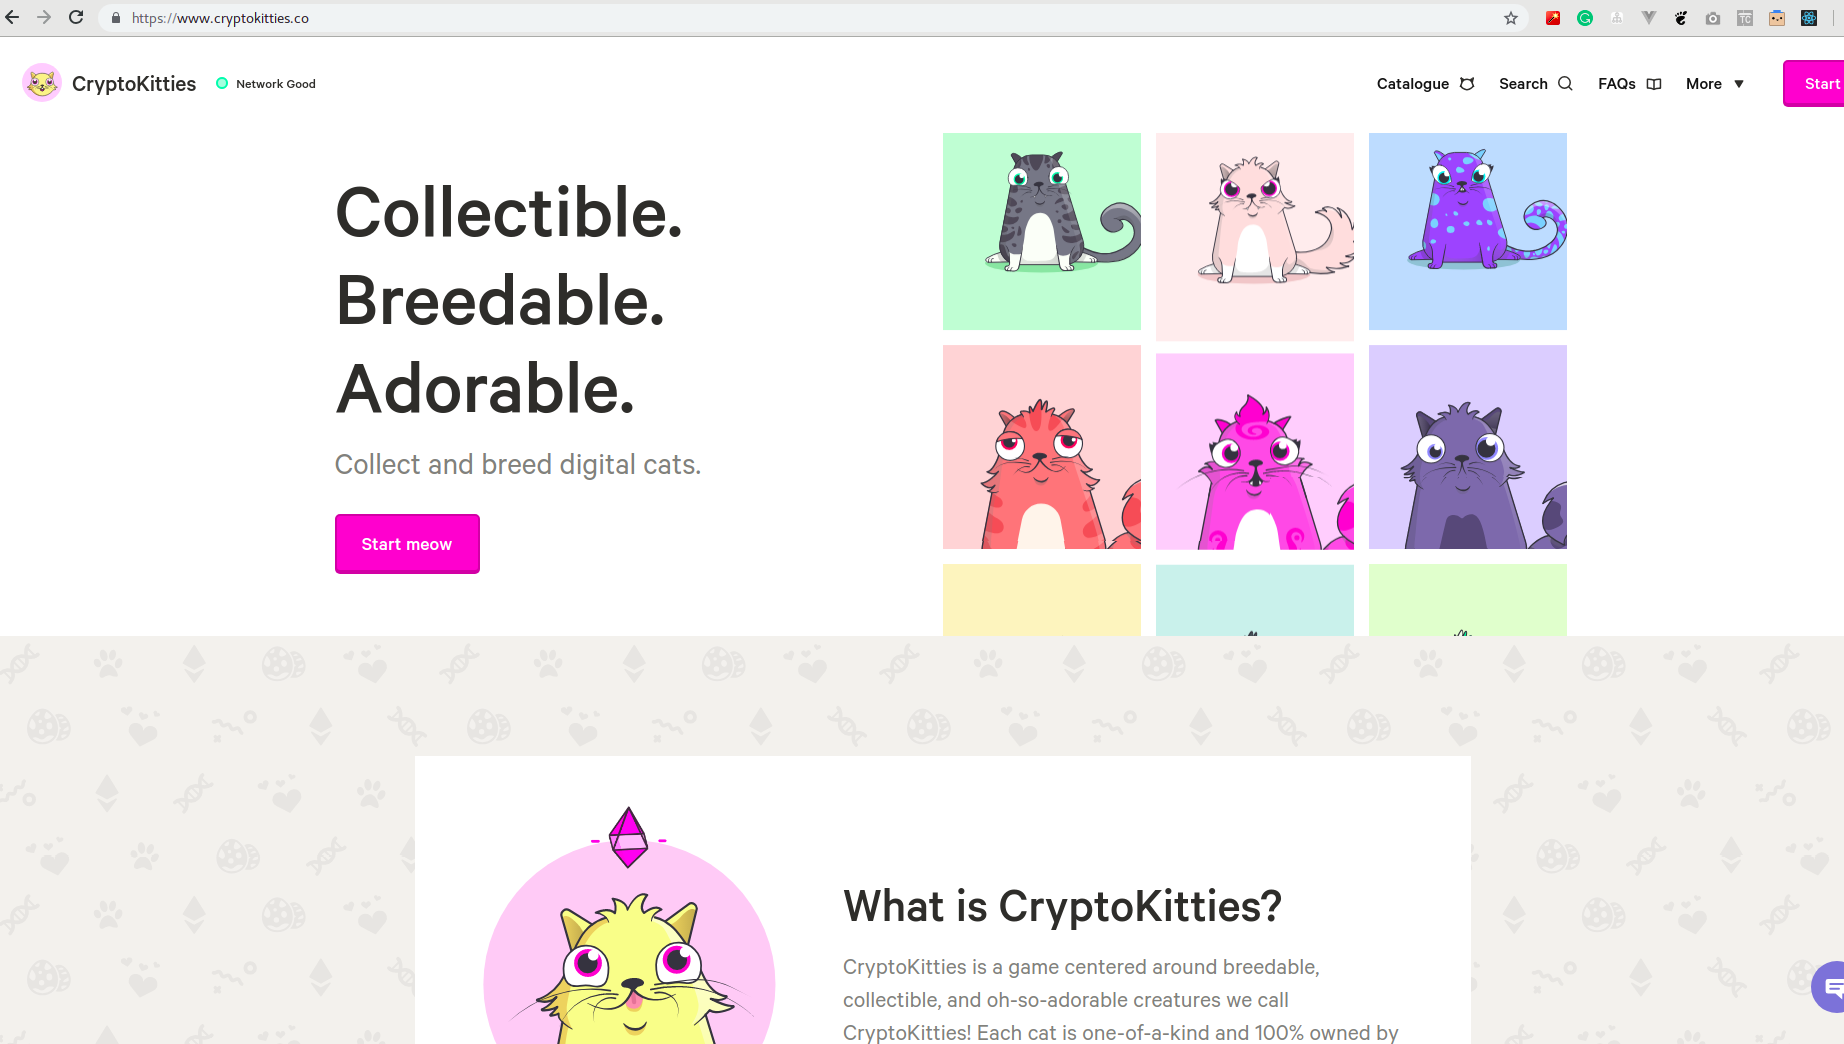
\includegraphics[width=0.8\textwidth]{criptokittieshome}
\caption[CriptoKitties]{Homepage de CriptoKitties al dia 01-12-2018 13:00}
\label{fig:criptokitties-home}
\end{figure}

\subsection{El "trilema"}
Una de las teorías de blockchain es que una red puede soportar solo dos de los siguientes:
seguridad, descentralización y escalabilidad sin perder terreno en el tercero restante.

Este "trilema" es un desafío de los desarrolladores Ethereum en su intento de mantener los
principios
básicos de una blockchain (descentralización y seguridad) al mismo tiempo que intentan escalar para
su adopción generalizada.



%********************************** %Fourth Section  *************************************
\section{Justificación y motivación} %Section - 1.2


\section{Objetivos de la investigación}
La presente investigación tiene dos objetivos principales: Por un lado, entender la base y funcionamiento
de una blockchain en general para luego pasar al estudio del ecosistema de Ethereum. Por el otro, ganar
entendimiento de los problemas de escalabilidad que se presentan en Ethereum (que recordemos están
presentes en toda blockchain) y presentar posibles soluciones que se encuentran en experimentación o en su
fase teórica.

\section{Preguntas de investigación}
¿Qué es Blockchain?

¿Qué es Ethereum?

¿Cómo funciona una base de datos distribuida?

¿Qué es el Ether y para qué se usa?

¿A qué se refiere el término "minar" en blockchain?

¿?

¿?


\section{Viabilidad}
A pesar de tener poco más de tres años en el mercado y encontrarse aún en fase experimental,
Ethereum cuenta con miles de documentos online, aplicaciones desarrolladas y open source, videos
conferenciales y otros recursos tanto educativos como profesionales. Además cabe destacar que 
cualquier persona tiene a dispocición el paper científico sobre Ethereum.

\nomenclature[z-DEM]{DEM}{Discrete Element Method}
\nomenclature[z-FEM]{FEM}{Finite Element Method}
\nomenclature[z-PFEM]{PFEM}{Particle Finite Element Method}
\nomenclature[z-FVM]{FVM}{Finite Volume Method}
\nomenclature[z-BEM]{BEM}{Boundary Element Method}
\nomenclature[z-MPM]{MPM}{Material Point Method}
\nomenclature[z-LBM]{LBM}{Lattice Boltzmann Method}
\nomenclature[z-MRT]{MRT}{Multi-Relaxation 
Time}
\nomenclature[z-RVE]{RVE}{Representative Elemental Volume}
\nomenclature[z-GPU]{GPU}{Graphics Processing Unit}
\nomenclature[z-SH]{SH}{Savage Hutter}
\nomenclature[z-CFD]{CFD}{Computational Fluid Dynamics}
\nomenclature[z-LES]{LES}{Large Eddy Simulation}
\nomenclature[z-FLOP]{FLOP}{Floating Point Operations}
\nomenclature[z-ALU]{ALU}{Arithmetic Logic Unit}
\nomenclature[z-FPU]{FPU}{Floating Point Unit}
\nomenclature[z-SM]{SM}{Streaming Multiprocessors}
\nomenclature[z-PCI]{PCI}{Peripheral Component Interconnect}
\nomenclature[z-CK]{CK}{Carman - Kozeny}
\nomenclature[z-CD]{CD}{Contact Dynamics}
\nomenclature[z-DNS]{DNS}{Direct Numerical Simulation}
\nomenclature[z-EFG]{EFG}{Element-Free Galerkin}
\nomenclature[z-PIC]{PIC}{Particle-in-cell}
\nomenclature[z-USF]{USF}{Update Stress First}
\nomenclature[z-USL]{USL}{Update Stress Last}
\nomenclature[s-crit]{crit}{Critical state}
\nomenclature[z-DKT]{DKT}{Draft Kiss Tumble}
\nomenclature[z-PPC]{PPC}{Particles per cell}
%!TEX root = ../thesis.tex
%*******************************************************************************
%****************************** Second Chapter *********************************
%*******************************************************************************

\chapter{Marco teórico}

\ifpdf
    \graphicspath{{Chapter2/Figs/}{Chapter2/Figs/PDF/}{Chapter2/Figs/}}
\else
    \graphicspath{{Chapter2/Figs/}{Chapter2/Figs/}}
\fi


\section{Blockchain}
Blockchain o cadena de bloques es un registro público de transacciones que se
mantiene mediante una red distribuida de computadores, que no requiere respaldo de
ninguna autoridad central o una tercera parte y que ofrece un esquema transaccional
libre de intermediarios, gracias al uso de algoritmos criptográficos. Puede compararse con el libro
de registros de contabilidad de una empresa en donde se registran todas las entradas
y salidas de dinero, aunque en este caso hablamos de un libro de acontecimientos
digitales que no requiere de un intermediario centralizado que identifique y certifique la
información, sino que está distribuida en múltiples nodos independientes entre sí que
la registran y la validan sin necesidad de que haya confianza entre ellos.

Esta cadena de bloques (blockchain) consta de tres componentes fundamentales: transacciones,
registro y un sistema que las verifica y almacena en bloques. Cada bloque se genera a través de un
software que registra cronológicamente la información sobre cuándo y en qué secuencia han tenido
lugar las transacciones, de allí deriva su nombre. 
Esta tecnología permite que se realicen las transferencias electrónicas de una manera segura sin la
presencia de un tercero de confianza, dando solución a la principal barrera técnica de las últimas
décadas para los desarrolladores tecnológicos, el problema del doble gasto.

Por fuera de Blockchain, las transferencias electrónicas requieren intermediarios financieros para
dar confianza y seguridad a la transacción. Los intermediarios financieros generan confianza y
seguridad, preservando un registro único y centralizado de las operaciones electrónicas que permite
controlar los saldos de los titulares de cuentas y, en última instancia, garantizar la autenticidad
de una transacción. Sin intermediarios, las unidades de valor electrónicas -pesos o dólares- pueden
ser copiados y usados dos veces, tal como cualquier documento digital puede ser copiado
indefinidamente. En Blockchain, una vez introducida la información, no puede ser borrada o
modificada, solo se podrán añadir nuevos registros y no será legitimada a menos que la mayoría de
los actores se pongan de acuerdo para hacerlo.

Se podría entender esta tecnología con fundamento en sus tres características generales de la
siguiente forma: i) Blockchain es una tecnología "sin confianza", lo que significa que por primera
vez en la historia, intercambios de valor a través de una red de computadores pueden ser
verificados, monitoreados y asegurados sin la presencia de un tercero de confianza o
de una institución central; ii) es una tecnología de autenticación y verificación, que permite de
forma más eficiente las transferencias de títulos y la verificación de propiedad y iii) por ser una
tecnología sin fronteras y sin fricción, puede proporcionar una más económica y rápida
infraestructura para el intercambio de unidades de valor.

Esta tecnología surgió como el soporte tecnológico del Bitcoin y luego fue adoptada por múltiples
sectores en donde existía la necesidad de un registro o de intercambio de valor, como se verá más
adelante. Para comprender el funcionamiento general del Blockchain, se explicará la primera versión
que sirvió de base para los desarrollos en los que se está trabajando en la actualidad.


\subsection{¿Cómo funciona?}
Veremos más sobre el funcionamiento de Ethereum en otros capítulos. Aquí se intentará explicar de 
manera generalizada el funcionamiento de una blockchain.

Para generar un contexto, supondremos que Alpha quiere transferir a Beta una determinada
cantidad de unidades de valor (Alguna criptomoneda, pesos, dólares, etc.) y que ambos tienen acceso
a una billetera o un monedero en el celular, un computador o una web que les permite enviar o
recibir la moneda. Cuando Alpha decide gastar sus unidades de valor, lo que realmente está haciendo
es enviar una instrucción de cambio a la base de datos informando que parte de sus unidades de
valor ahora pertenecen a Beta. Esta instrucción es difundida en la red verificando que Alpha tiene
recursos para pagar y, si todo se encuentra correcto, se compila con otras transacciones
en un bloque con información relativa a los últimos diez minutos.
Este bloque mezcla la información de las direcciones de las partes involucradas en cada
transacción, la cantidad de unidades de valor en movimiento y una marca de tiempo, y luego las
procesa a través de una función llamada Hash. Esta función es un algoritmo criptográfico, que se
encarga de condensar en un único digito de 64 caracteres información de cualquier extensión.
Por ejemplo, el hash (encriptado con el algoritmo SHA-256) para la palabra “blockchain” sería
EF7797E13D3A75526946A3BCF00DAEC9FC9C9C4D51DDC7CC5DF888F74DD434D1 y el de “Blockchain”
625DA44E4EAF58D61CF048D168AA6F5E492DEA166D8BB54EC06
C30DE07DB57E1. Preste especial atención que ante cambios como la capitalización de una letra o la
longitud del texto, el hash es completamente diferente.

Este hash se combina con la solución-hash del bloque anterior, y se convierte en el encabezado del
bloque nuevo que se encuentra en validación. A su vez este es la base de un problema matemático que
se resuelve usando de nuevo la función Hash. La respuesta a este acertijo es solucionado por la red
en un proceso de prueba y error. Cuando finalmente algún nodo de la red encuentra la solución, esta
es compartida con el resto para su validación, en un proceso llamado “proof of work” (prueba de
trabajo). Después que ha sido aprobada por la mayoría de la red, el bloque es añadido a la cadena y 
con ello todas las transacciones contenidas en él, incluido el pago de Alpha hacia Beta.

La blockchain establece la confianza entre dos partes en una transacción a través de un libro de 
contabilidad público descentralizado y un mecanismo criptográfico que garantiza que las 
transacciones no pueden cambiarse después de materializadas.

\section{Ethereum}
Ethereum aparece a finales del año 2013 en un paper publicado por Vitalik Buterin con el objetivo
de proveer un sistema descentralizado capaz de correr aplicaciones casi sin límite de capacidades.

Ethereum es una red peer-to-peer (p2p) de máquinas virtuales que cualquier desarrollador puede
utilizar para ejecutar aplicaciones distribuidas (dApps). Estos programas informáticos pueden ser
cualquier cosa, pero la red está optimizada para llevar a cabo reglas que se ejecutan mecánicamente
cuando se cumplen ciertas condiciones, como un contrato. Ethereum utiliza su propia blockchain
pública descentralizada para almacenar, ejecutar y proteger criptográficamente estos contratos. 
Cada computadora de su red descarga una pequeña máquina virtual para sincronizarse con la
blockchain de Ethereum y volver a estar disponible para ejecutar contratos. Esta red distribuida de
computadoras proporciona convenientemente la seguridad, confiabilidad y potencia de computación
necesarias para llevar a cabo los arreglos diseñados. Por supuesto, esta red de consenso no es
gratuita ni privada, por lo que los desarrolladores sólo la utilizan para llegar a un consenso
sobre los resultados y cuando sus datos pueden ser públicos.

La intención de Ethereum es crear un protocolo alternativo para la construcción de dApps,
proporcionando un conjunto diferente de compensaciones que se cree serán muy útiles para una gran
clase de aplicaciones descentralizadas, con especial énfasis en situaciones en las que el tiempo de
desarrollo rápido, la seguridad para aplicaciones pequeñas y poco utilizadas, y la capacidad de las
 diferentes aplicaciones para interactuar muy eficientemente, son importantes.
Ethereum hace esto construyendo lo que es esencialmente la última capa fundacional abstracta: una
blockchain con un lenguaje de programación Turing completo integrado, que permite a cualquiera
escribir contratos inteligentes y aplicaciones descentralizadas donde puede crear sus propias
reglas arbitrarias para la propiedad, formatos de transacción y funciones de transición de estado.


\subsection{Fíat Currency (dinero fiduciario)}
Comúnmente se dice que el bitcoin no está respaldado por nada, y eso es cierto. Las monedas fiat
modernas tampoco están respaldadas por nada, sin embargo, son diferentes: endosados
por un gobierno, una moneda fiduciaria es mantenida por defecto por cualquiera que pague impuestos
y compre bonos del Estado. Algunas ventas internacionales de materias primas están denominadas en
dólares, también (por ejemplo, el petróleo) dando a la gente otra razón para retener dólares.

En el caso de las criptomonedas, persisten los problemas de adopción. Hoy en día, estos tokens
digitales siguen siendo una capa de pago público, rápido y seguro en la parte superior del sistema
de dinero fiduciario existente; un despliegue experimental que podría algún día crecer para
reemplazar los pagos centralizados utilizadas hoy en día por empresas como Visa y MasterCard.

Se vislumbran grandes posibilidades en el horizonte, ya que los gobiernos y el sector privado s
encuentran en una situación difícil. Los inversores institucionales empiezan a crear grandes
mercados para los productos y servicios financieros denominadas en criptomonedas. Los bancos
centrales pueden incluso adoptar esta tecnología. Al menos un país ha emitido un dólar digital
utilizando el software Bitcoin: Barbados. Otros están investigando activamente el prospecto.


\subsubsection{Ether}
Hoy en día, Bitcoin (denotado por el símbolo BTC) es utilizado por personas, gobiernos y empresas
para transferir valor y comprar productos o servicios. Cada vez que envían bitcoins, pagan una
pequeña cuota a la red, que está denominada en bitcoins. Ether, denotado por el símbolo ETH, se
puede utilizar de forma similar. Para entender el camino a seguir, se necesita saber algunas cosas.

Primero, el ether tiene otro uso: puede pagar para ejecutar programas en la red de Ethereum.
Estos programas pueden transferir el ether ahora, o en el futuro, o cuando se cumplan ciertas
condiciones (especificadas en los contratos).
Debido a su capacidad de pagar por la ejecución de transacciones en el futuro, el ether puede
también ser considerado un producto básico, como el combustible para que la red ejecute
aplicaciones y servicios. Por lo tanto, tiene una dimensión adicional de valor intrínseco sobre los
bitcoins; no es sólo una reserva de valor.

Hoy en día, el abrumador uso de las monedas fiduciarias podría sugerir que
las criptomonedas son "peor dinero", es decir, más propensas a la inutilidad a largo plazo.
Y sin embargo, los bitcoins y el ether son famosamente acaparados por los poseedores, e incluso
mantenidos en un fideicomiso por al menos una compañía hasta el momento de escribir esto:
Grayscale, una subsidiaria de Digital Currency Group es un buen ejemplo.
Mientras tanto, los bancos centrales de Occidente experimentan con tipos de interés cercanos a cero
y flexibilización cuantitativa, también conocida como impresión de dinero, en una situación cada
vez más peligrosa y desesperada por mantener la inflación y la deflación bajo control.

Con la recompensa de bitcoin reduciéndose a la mitad cada cuatro años, la política monetaria
mundial se ve afectada. En general la incertidumbre económica, y la disminución de la confianza en
las monedas fiduciarias, enormes sumas de dinero latente en criptomonedas "acaparadas" están siendo
arrastradas al mercado por los precios más altos del servicio de demanda genuina. Esto se refleja
en los precios cada vez mayores de la mayoría de los tokens criptográficos, por muy volátiles que
sean sus precios intradía. Este acto de equilibrio entre acaparadores, especuladores, y
"derrochadores" crea un mercado próspero y saludable para la criptomoneda, y sugiere que
los criptokens como una clase de activos ya están sirviendo a los propósitos del dinero, y mucho
más.


\subsection{Protocolos}
Por definición, un protocolo en informática y telecomunicaciones es un sistema de normas que
regulan la comunicación entre dos o más sistemas que se transmiten información a través de 
diversos medios físicos.

Los protocolos pueden variar en gran manera, sin embargo, suelen tener al menos una de las 
siguientes propiedades:

\begin{itemize}
\item Detección de la conexión física subyacente.
\item Negociación de características de conexión.
\item Política de corrección de errores.
\item Establecimiento de la conexión y su término.
\item Qué hacer en caso de pérdida repentina de la conectividad.
\item Estrategias de seguridad o cifrado.
\item Formato de los mensajes.
\end{itemize}


\subsubsection{Ethereum Wire Protocol}
%@TODO

\subsection{Smart Contracts}
El término smart contract hace referencia a cualquier contrato que se ejecuta por sí mismo
automáticamente sin que medien terceros entre los participantes individuales. Los smart contracts
se escriben como programas informáticos en lugar de como lenguaje legal sobre documentos impresos.
El programa puede definir reglas y consecuencias estrictas del mismo modo que lo haría un documento
legal tradicional, pero a diferencia de los contratos tradicionales, también puede tomar
información como input, procesarla según las reglas establecidas en el contrato y adoptar cualquier
medida que se requiera como resultado de ello.

El concepto lo definió en 1994 el criptógrafo Nick Szabo, pero en la práctica no se hizo realidad
porque la infraestructura tecnológica necesaria para apoyarlo aún no existía. En la actualidad, con
la llegada de los protocolos de cifrado y el blockchain la situación cambió y, como resultado, la
idea ha vuelto a renacer.

En resumen, los contratos inteligentes son scripts modulares, repetibles y autónomos que
normalmente se ejecutan en una blockchain y representan promesas unilaterales de proporcionar una
tarea informática determinada. Estos scripts se almacenan en la blockchain, en una dirección
específica que se determina cuando se implementan los contratos en la blockchain. Cuando se produce
un evento contemplado en el contrato, se envía una transacción a esa dirección y la máquina virtual
distribuida ejecuta los códigos de operación del script (o cláusulas) utilizando los datos enviados
con la transacción.

Los contratos inteligentes pueden estar codificados de modo que reflejen cualquier tipo de lógica
empresarial basada en los datos: desde acciones tan sencillas como votar por una publicación en un
foro hasta acciones con un mayor nivel de complejidad, como garantías de préstamos y contratos de
futuros, así como acciones sumamente complejas como la fijación de prioridades de pago en una nota
estructurada.


\subsection{Solidity programming language}
Solidity es un lenguaje de programación de alto nivel "contract-oriented" usado para escribir
programas (smart contracts), que serán ejecutados por la EVM (Ethereum Virtual Machine). Su
sintaxis es muy similar a lenguajes como JavaScript o C.
Este lenguaje es una mezcla de convenciones de networking, lenguaje ensamblador, y desarrollo web.

Veremos más sobre él en capítulos posteriores.

\subsection{Base de datos distribuida, ¿Dónde están los datos?}
En Ethereum, la red es la base de datos. Todos los datos de los usuarios están almacenados en 
cada nodo de la red. Todas las transacciones en Ethereum se almacenan en la blockchain, un
historial cambios de estado es almacenados en cada nodo de Ethereum.

Cuando un usuario paga por el tiempo de computación en la red Ethereum, esto incluye el costo
de ejecutar la transacción y para el almacenamiento de los datos incluidos en su contrato
inteligente. (Si el contrato se hace más pequeño después de ejecutarse, el usuario recibirá un
reembolso parcial en forma de tarifa de transacción reducida.)

Tan pronto como se ejecute el smart contract y la tarifa en ether sea pagada, los datos serán
incluídos en el siguiente bloque. Debido a que la red Ethereum requiere que todos los nodos
mantengan el estado de todos los contratos, cualquier nodo puede consultar a la base de datos
local. Esto es sumamente poco escalable!



%!TEX root = ../thesis.tex
%*******************************************************************************
%****************************** Third Chapter **********************************
%*******************************************************************************
\chapter{Método}

% **************************** Define Graphics Path **************************
\ifpdf
    \graphicspath{{Chapter3/Figs/Raster/}{Chapter3/Figs/PDF/}{Chapter3/Figs/}}
\else
    \graphicspath{{Chapter3/Figs/}{Chapter3/Figs/}}
\fi

\section{Estudio de tecnologías}

\subsection{Proceso de aprendizaje}

Para definir el proceso de aprendizaje llevado a cabo pienso que es necesario hacer una división en
lo que claramente define mi conocimiento en el antes de comenzar este informe y lo que es el
durante y el después. Durante el desarrollo del informe y la aplicación se pueden separar tres
grandes conceptos: Node.js, Blockchain y Ethereum.

Por un lado, Node.js es una tecnología con la que trabajo a diario hace más de dos años y por este
motivo no será el centro de atención a lo largo del informe. Si bien los contratos que se escriban, 
testeen y deployen lo harán en principio sobre una plataforma escrita en Node.js, se le dará suma
importancia a lo incurrido en los otros dos conceptos.

Por otro lado, Blockchain y Ethereum son dos conceptos completamente ajenos a mi experiencia. Si 
bien se oyen a diario cada vez más seguido, jamás antes había siquiera leído un informe o un libro
sobre ninguno de estos dos conceptos. Este hecho de escucharlos y leerlos todos los días en 
noticias de tecnología me hizo pensar en profundizar en ellos para conocer su funcionamiento 
interno, sus posibles aplicaciones y lograr junto con este informe, crear y deployar contratos 
inteligentes en las redes de pruebas, teniendo pleno conocimiento de lo que está sucediendo en el 
detrás de escena y habiendo intervenido todo lo que en mi responsabilidad quedaba hacerlo.

Dado que a lo largo de la facultad no se ha visto contenido alguno relacionado a Blockchain y 
Ethereum, todo lo aprendido en este proceso fue adquirido de libros, artículos de blogs 
técnicos, los propios papers oficiales de Bitcoin y Ethereum, videos de conferencias, videos 
académicos, informes y otras fuentes de menor importancia.

El proceso de aprendizaje comienza mediados del mes de Noviembre de 2018 donde se comienza a 
recolectar todos los recursos "en crudo" considerados importantes para la finalidad del informe.
Es decir, libros, artículos, informes, papers, cursos, conferencias, etc. Los recursos aquí 
buscados fueron, en números, un 85\% sobre Blockchain y Ethereum y el 15\% restante sobre como
comunicar la plataforma de Node.js con los contratos inteligentes y los nodos de las redes de 
prueba de Ethereum.

Ya comenzado el mes de Diciembre, se procedió a filtrar todos los recursos en crudo para dejar
lo considerado más importante y que me iba a dar más conocimiento de los temas para llevar adelante
el informe y el proyecto.

Rondando mediados de Diciembre y luego de haber incurrido en algunos libros, informes y videos 
académicos, se está en condiciones de comenzar a escribir una aplicación combinando Node.js, 
Ethereum y Blockchain. A partir de este momento el progreso realizado se verá reflejado luego 
en la sección "Estado alcanzado" más adelante.


\subsection{Estado alcanzado}
La etapa de aprendizaje inicial comenzó algo lenta por cuestiones de organización pero pasado
el tiempo se fue ganando velocidad y adquiriendo conocimientos a la par que se investigaba y 
desarrollaba.

Al día de hoy, próximo a finalizar, considero realmente un éxito el estado alcanzado porque 
se comenzó sabiendo absolutamente nada de Blockchain y Ethereum y se pudo culminar con el 
desarrollo de una aplicación que utilice estas tecnologías habiendo absorvido los conocimientos
necesarios.

\section{Proceso de desarrollo}

\subsection{Puesta en marcha del entorno de trabajo}

Para llevar adelante tanto el presente informe como la aplicación, se utilizó una única estación
de trabajo descripta a continuación:

\begin{itemize}
\item Modelo: Ultrabook Dell Latitude E7270
\item Memoria RAM: 8GB DDR4 2133mhz.
\item CPU: Intel Core i7 6600U @ 2.60GHz.
\item Almacenamiento: Disco SSD LITEON L8H-256V2G-11 M.2 2280 256GB.
\item Sistema Operativo: Debian GNU/Linux 9.4 (stretch) 64 bits.
\end{itemize}

Enumeraré a continuación lo que se debió instalar en dicha estación de trabajo. No daré
practicamente detalles debido a que de muchos puntos se ha hablado en otras secciones:

\begin{itemize}
\item LaTeX https://packages.debian.org/stretch/texlive-full
\item Texmaker https://packages.debian.org/jessie/tex/texmaker
\item nvm (Node Version Manager) https://github.com/creationix/nvm
\item Node.js v10 LTS https://nodejs.org/ (posteriormente luego de hacer pruebas, se instalará definitivamente la versión v8 LTS para el proyecto
\item MetaMask https://metamask.io/
\item Módulos externos de Node.js:
	\begin{itemize}
		\item Mocha https://github.com/mochajs/mocha
		\item Ganache CLI https://github.com/trufflesuite/ganache-cli
		\item Truffle HD Wallet Provider https://github.com/trufflesuite/truffle-hdwallet-provider
		\item Web3 https://github.com/ethereum/web3.js/
		\item Solc (compilador de código Solidity) https://github.com/ethereum/solc-js
	\end{itemize}
\item Módulos externos de y para trabajar con React
	\begin{itemize}
		\item React
		\item React DOM
		\item React Router DOM
		\item @babel/core (todos los paquetes instalados de @babel son utilizados para transpilar código escrito en nuevos estándares para que sean compatibles con navegadores más antiguos)
		\item @babel/plugin-proposal-class-properties
		\item @babel/preset-env
		\item @babel/preset-react
		\item @babel/polyfill
		\item Babel Loader
		\item CSS Loader
		\item Webpack
		\item Webpack CLI
		\item Webpack Dev Server
		\item Style Loader
		\item HTML Webpack Plugin
	\end{itemize} 
\end{itemize}

\subsection{Product Backlog}
En esta sección se encontrarán todas las tareas llevadas a cabo desde el mismísimo principio del
presente informe cuando siquiera sabía lo que era Ethereum. Quiero destacar que en principio 
realicé una división de las tareas en tres categorías que me ayudan a separar y organizar un poco
mejor lo que este trabajo conlleva. 

Por un lado estarán las tareas identificadas como \textbf{\textit{[BIBLIOGRAFÍA]}}, las cuales 
representan todas aquellas tareas que se identifiquen con la búsqueda de material, investigación,
lectura y no conlleven un fin estrictamente práctico más que el estudio del material recolectado y
elegido. Por otro lado están las tareas de \textbf{\textit{[INFORME]}}, las cuales representan 
todas las tareas directamente relacionadas con el presente informe, ya sea su creación, escritura, 
revisiones, mantenimiento, etc. Y por último estarán las tareas presentadas como 
\textbf{\textit{[APP]}}, que serán las que estén ligadas al desarrollo de la aplicación que nace
de toda la investigación previa de Ethereum y su ecosistema.

Habiendo aclarado lo anterior, presento el backlog a continuación:

\begin{itemize}
\item \textbf{[BIBLIOGRAFÍA]} Investigar y guardar material en crudo sin filtrar sobre Blockchain, Ethereum y la pposible participación de Node.js en su ecosistema (1)
\item \textbf{[BIBLIOGRAFÍA]} Evaluar en detalle el material recolectado y filtrar únicamente lo
que se relacione directamente con los conceptos core que se van a llevar adelante y tengan el
debido respaldo profesional de la comunidad: Blockchain y Ethereum (2)
\item \textbf{[BIBLIOGRAFÍA]} Leer comprensivamente el paper de Bitcoin 
(https://www.bitcoin.com/bitcoin.pdf) (3)
\item \textbf{[BIBLIOGRAFÍA]} Leer comprensivamente el paper de Ethereum 
(https://github.com/ethereum/wiki/wiki/White-Paper) (4)
\item \textbf{[BIBLIOGRAFÍA]} Estudiar video del fundador de Ethereum en conferencia 
https://www.youtube.com/watch?v=66SaEDzlmP4 (5)
\item \textbf{[BIBLIOGRAFÍA]} Leer el siguiente artículo 
https://medium.com/@mattcondon/getting-up-to-speed-on-ethereum-63ed28821bbe (6)
\item \textbf{[BIBLIOGRAFÍA]} Leer la documentación de Solidity https://solidity.readthedocs.io/en/develop/ (7)
\item \textbf{[BIBLIOGRAFÍA]} Leer capítulos [1, 3] y [5, 7] del libro "Ethereum Smart Contract Development" https://www.amazon.com/gp/product/B077YSHRWW (8)
\item \textbf{[BIBLIOGRAFÍA]} Revisar recursos expuestos en el siguiente articulo 
https://medium.com/@robbertvermeulen/learn-solidity-the-ethereum-smart-contract-programming-language-7f106fc26d6 (9)
\item \textbf{[BIBLIOGRAFÍA]} Leer el siguiente artículo para continuar comprendiendo cómo y dónde
se guardan los datos en Ethereum https://hackernoon.com/getting-deep-into-ethereum-how-data-is-stored-in-ethereum-e3f669d96033 (10)
\item \textbf{[BIBLIOGRAFÍA]} Leer libro "Mastering Ethereum" https://github.com/ethereumbook/ethereumbook (11)

\item \textbf{[INFORME]} Instalar LaTeX y Texmaker (12)
\item \textbf{[INFORME]} Clonar y configurar plantilla para el informe (https://github.com/kks32/phd-thesis-template) (13)
\item \textbf{[INFORME]} Crear índice tentativo que además me servirá personalmente como guía (14)
\item \textbf{[INFORME]} Crear repositorio en Github para el informe en LaTeX (https://github.com/Lzok/ethereum-report) (15)
\item \textbf{[INFORME]} Trabajar sobre el capítulo 1 (16)
\item \textbf{[INFORME]} Trabajar sobre el capítulo 2 (17)
\item \textbf{[INFORME]} Trabajar sobre el capítulo 3 (18)
\item \textbf{[INFORME]} Trabajar sobre el capítulo 4 (19)

\item \textbf{[APP]} Crear repositorio en Github para la app (20)
\item \textbf{[APP]} Instalar nvm y Node.js v10 LTS (21)
\item \textbf{[APP]} Set up del editor de código, VS Code. (22)
\item \textbf{[APP]} Instalar todos los módulos necesarios para el proyecto (23)
\item \textbf{[APP]} Evaluar módulos para test runner: Mocha o Jest? (24)
\item \textbf{[APP]} Instalar y configurar test runner elegido del punto anterior (25)
\item \textbf{[APP]} Escribir un contrato sencillo para probar Remix remix.ethereum.org (26)
\item \textbf{[APP]} Hacer una cuenta en Infura (https://infura.io/) y obtener la access key (27)
\item \textbf{[APP]} Hacer pruebas para evaluar la versión definitiva de Node para usar en el
proyecto debido a que el entorno de Ethereum es muy volátil en cuanto a las versiones del
ecosistema. Posteriormente, instalar la versión de Node más estable para el proyecto. (28)
\item \textbf{[APP]} Hacer el contrato Project en el IDE Remix para investigar qué versión del
compilador Solidity es compatible con el código escrito y cerciorarse de que compile sin problemas.
(29)
\item \textbf{[APP]} Una vez que el contrato Project esté funcionando, se debe hacer el contrato
ProjectBuilder siguiendo el mismo procedimiento (30)
\item \textbf{[APP]} Pasar los contratos escritos a un directorio dentro del proyecto y escribir
un script Node para que el módulo solc pueda compilarlos localmente. (31)
\item \textbf{[APP]} Escribir un script Node para deployar los contratos en la red privada de 
pruebas Rinkeby (33)
\item \textbf{[APP]} Escribir el código para consumir los métodos del contrato ProjectBuilder (34)
\item \textbf{[APP]} Escribir el código para conectarse al contrato a través de Web3 (35)
\item \textbf{[APP]} Hacer el set up del entorno de React, React Router, Webpack y Babel en el
proyecto (36)
\item \textbf{[APP]} Hacer componente para la pagina de Index en React (HTML + JS + CSS) (37)
\item \textbf{[APP]} Hacer los componentes Header y Footer (HTML + JS + CSS) (38)
\item \textbf{[APP]} Hacer el formulario para crear un nuevo proyecto en React con la logica
necesaria para enviar la informacion al smart contract deployado (HTMl + JS + CSS) (39)
\item \textbf{[APP]} Hacer el componente que muestre el detalle de un proyecto (HTML + JS + CSS) (40)
\item \textbf{[APP]} Hacer el componente para que un usuario pueda ser backer de un proyecto junto
con la logica necesaria (HTMl + JS + CSS) (41)
\item \textbf{[APP]} Hacer el componente para que el owner del proyecto cree un nuevo “payment”
junto con la logica necesaria (HTML + JS + CSS) (42)
\item \textbf{[APP]} Hacer componente para mostrar un listado de los payments (index) y su estado
(pendiente, rechazado, finalizado) (HTML + JS + CSS) (43)
\item \textbf{[APP]} Hacer componente para que los backers aprueben o desaprueben los pagos (HTML +
 JS + CSS) (44)

\end{itemize}

\subsection{Semana 0 o "kick off"}
Véase que nombro semana y no sprint como comúnmente se nombra a los períodos de trabajo en los 
cuales al final de cada uno se entrega una pieza funcional del proyecto en las metodologías ágiles
(o esa es la intención), el motivo de esta nomenclatura elegida es que al trabajar individualmente 
sin un equipo de personas y cargando con responsabilidades de la vida diaria y profesional no puedo
garantizar atenerme estrictamente a los planes, exigencias y entregas que plantean los sprints de 
trabajo en las metodologías ágiles. Por estos motivos, elegí ver y plantear los progresos que se 
lograron semanalmente durante la realización del proyecto.

En la semana 0 traté de dar algo de forma a mi "framework" de trabajo para estudiar
y realizar el presente informe y la app con la que culminaría lo que sería una primer etapa
concluída del aprendizaje de las tecnologías mencionadas. Algunas de las formas de trabajo 
establecidas fueron:

\begin{itemize}
\item Dedicar un promedio de al menos 2 (dos) horas diarias al proyecto en días de semana y 3
(tres) horas los fines de semana.
\item Al finalizar cada semana se registrarán los avances y nuevos conocimientos adquiridos.
\item El product backlog no estará dividido bajo ninguna estructura estricta ni cronológica.
\item A lo largo de las primeras cuatro semanas se priorizarán las actividades con el rótulo de 
\textbf{BIBLIOGRAFÍA} e \textbf{INFORME}.
\item A partir de la quinta semana idealmente, ya se comenzarán con las actividades con el rótulo
de \textbf{APP} y se continuará de aquí en más trabajando en paralelo con actividades de los tres
rótulos hasta concluir el proyecto.
\item El método de trabajo en el repositorio del informe sería crear una branch nueva por cada
capítulo, utilizando la branch \textit{master} como base.
\item El método de trabajo en el repositorio de la app sería crear una branch por cada feature
que se realice, utilizando la branch \textit{dev} como base de éstas y la branch \textit{master}
como la que contenga versiones estables y mínimente funcionales de la app.
\end{itemize}

\subsection{Semana 1}
La primer semana la dediqué enteramente a filtrar todo el grueso de links y bibliografía para
seleccionar a base de cuáles trabajar a lo largo del proyecto. Cabe destacar que esto no será 
definitivo ya que a lo largo del proyecto será muy común que surjan nuevos recursos que terminarán
siendo usados para el informe. Tickets (1) y (2).

\subsection{Semana 2}
Durante la segunda semana realicé la lectura de los capítulos requeridos en el ticket (8) del 
libro "Ethereum Smart Contract Development", la lectura del artículo mencionado en el ticket (6) y
la lectura de la documentación de Solidity propuesta en el ticket (7). Además, investigué los
recursos propuestos en el ticket número (9), el cual sugirió repositorios de Github interesantes
para consultar más adelante.

\subsection{Semana 3}
En esta semana se procedió a la lectura del paper de Bitcoin (3), el paper de Ethereum (4),
 la vista del video de Vitalik en conferencia (5), la lectura del artículo mencionado en el 
 ticket (10) y de los primeros dos capítulos del libro "Mastering Ethereum" (11).
 
\subsection{Semana 4}
Se continuó con la lectura de tres capítulos del libro "Mastering Ethereum" (11), se comenzó 
con la instalación de la suite de LaTeX para escribir el informe instalando LaTeX y el editor 
de texto llamado Texmaker (12), se clonó y configuró la plantilla de LaTeX seleccionada para 
hacer el informe y se configuró para las propias necesidades (13).

Además, se hizo un índice tentativo que sirve como guía para el desarrollo del informe (14), 
se creó el repositorio en Github para el informe (15), y por último se comenzó la escritura del
capítulo 1 (una escritura a modo de borrador) (16).


\subsection{Semana 5}
Durante esta semana se comenzó con trabajo relacionado al desarrollo de la app. Lo que se hizo fue
instalar NVM junto con la versión 10LTS de Node.js (21), hacer el set up del editor de código elegido
para trabajar (22), instalar los módulos necesarios para llevar adelante el proyecto con NPM (23),
se escribió un contrato de prueba en la plataforma Remix para comprobar que funcionase según lo
debido (26) y además se la cuenta en Infura.io para obtener la access key (27).

\begin{figure}[htbp!] 
\centering    
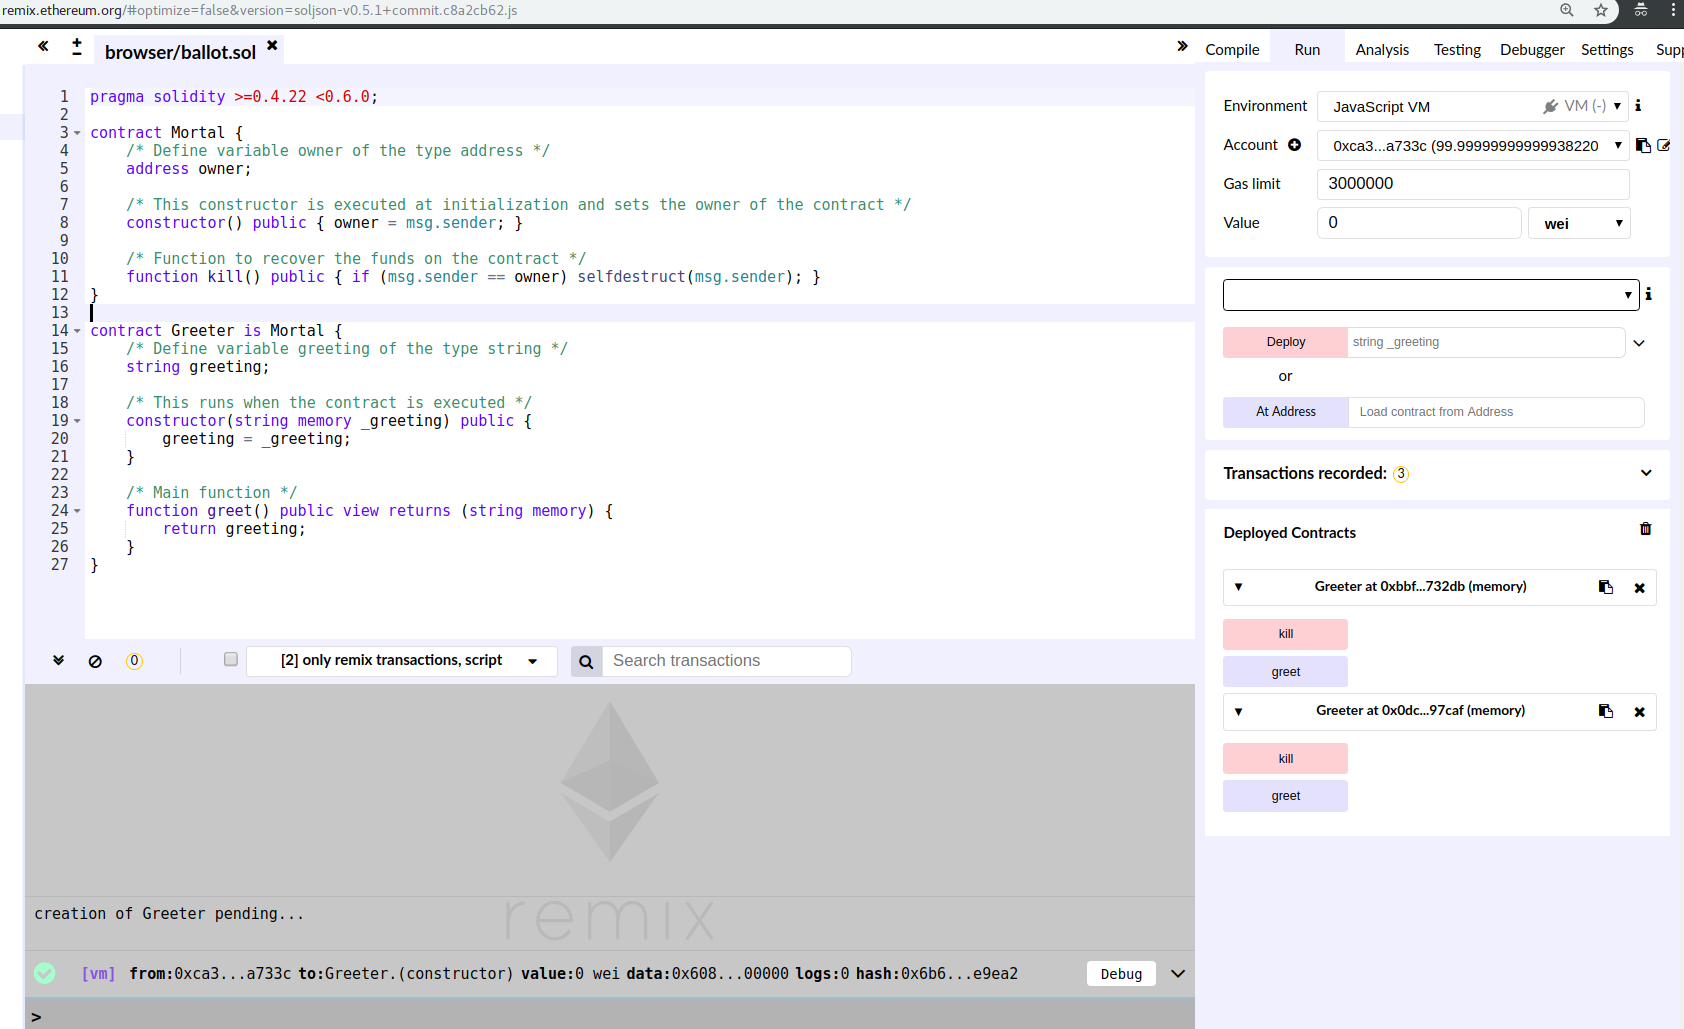
\includegraphics[width=0.8\textwidth]{contract-test}
\caption[contracttest]{Contrato sencillo con el único fin de probar Remix. (26)}
\label{fig:contract-test}
\end{figure}

\begin{figure}[htbp!] 
\centering    
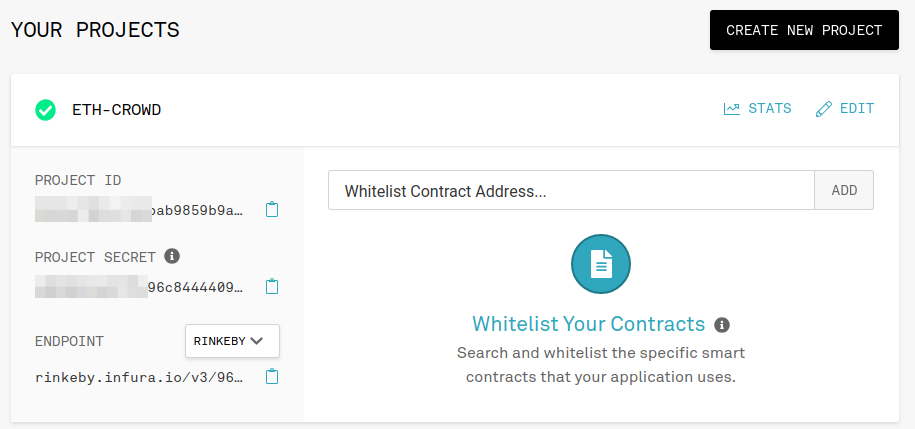
\includegraphics[width=0.8\textwidth]{infura-key}
\caption[infurakey]{Sección de la cuenta de Infura donde podemos obtener la access key. (27)}
\label{fig:infura-key}
\end{figure}

\subsection{Semana 6}
Se trabajó en el capítulo 2 del informe (17). Se creó el contrato Project en el IDE Remix
utilizando una versión de pragma solidity >=0.4.22 <0.6.0 y la versión de compilador
0.5.1+commit.c8a2cb62.Emscripten.clang (29). Se creó también el contrato ProjectBuilder con las 
mismas versiones utilizadas en el contrato Project (30).

En este punto del desarrollo debe decirse que ambos contratos compilan y se comportan correctamente
siendo utilizados en la plataforma Remix.

\subsection{Semana 7}
Durante esta semana se trabajó sobre los capítulos 1 y 2 del informe. Además, fue durante esta
semana donde comenzaron los problemas con las versiones de Node, Solidity, compiladores y librerías
utilizadas.

Como se dijo antes, durante la semana 6 se crearon los contratos Project y ProjectBuilder. Al 
comienzo de la semana 7 se comenzó la tarea de escribir un script de Node para poder compilar
los contratos con la librería \textit{solc v0.5.2} antes de deployarlos a la red (31). Luego de 
algunas horas investigando en la documentación de la librería y haciendo pruebas, logré compilar
lo que a simple vista parecía lo correcto para luego ser deployado a la red Rinkeby.

Teniendo el script compilando los contratos, se procedió a crear el script en Node para deployar
éstos a la red Rinkeby con la librería \textit{web3 v1.0.0-beta.38}. El script es sencillo, consta
de unas diez líneas de código pero sin embargo aquí es donde me topé con una pared de 
incompatibilidades. Detecté que el stack que la causaba eran las mencionadas versiones de 
\textit{solc} y \textit{web3} sumadas a Node v10. En los siguientes dos gráficos se puede ver
cómo el deploy entraba en un loop infinito contra la API de Infura, logrando llegar a más de mil
quinientos llamados al método \textit{eth\_getTransactionReceipt}. La llamada a este método es 
crucial debido a que en la respuesta (que nunca se pudo obtener correctamente) nos será devuelta
la dirección donde se deployó el contrato. Esta dirección le dirá luego a Node y React dónde tienen
que ir a buscar los métodos para ejecutar.

\begin{figure}[htbp!] 
\centering    
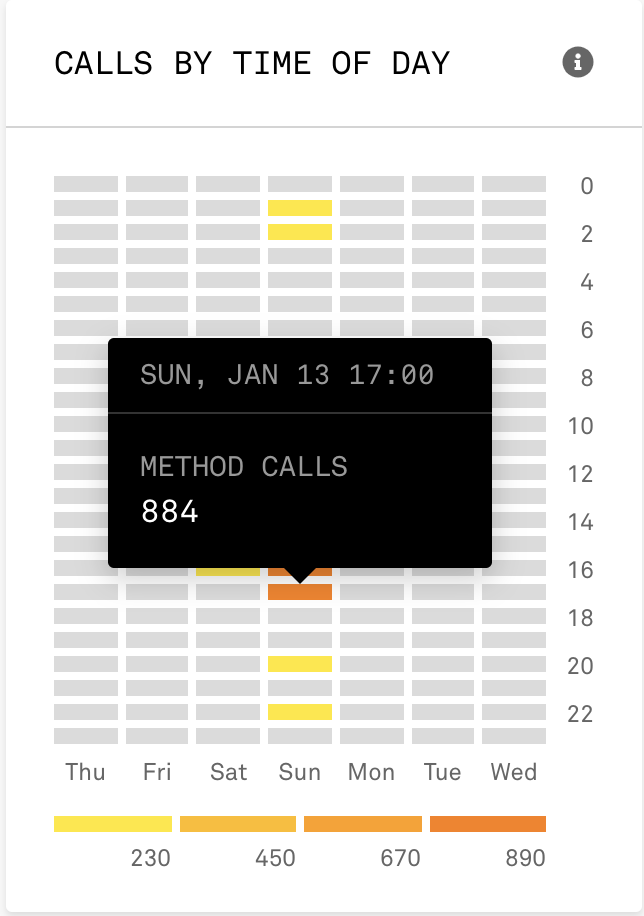
\includegraphics[width=0.8\textwidth]{infura-calls-1}
\caption[infuracalls1]{Se puede ver que entre las 16 y 17 horas (a la derecha) se produjeron un aproximado de 1760 llamados a la API de Infura.}
\label{fig:infura-calls-1}
\end{figure}

\begin{figure}[htbp!] 
\centering    
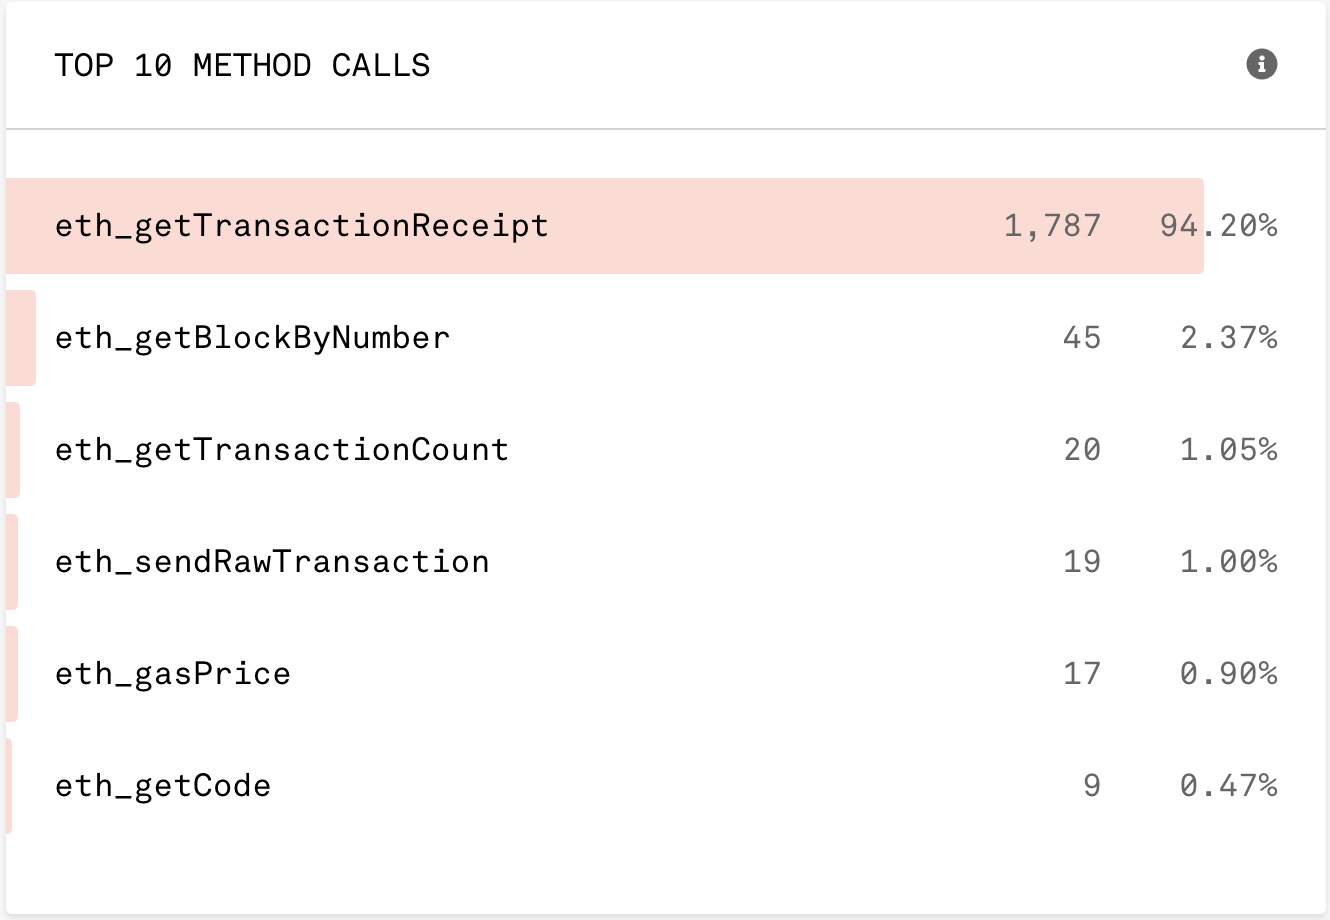
\includegraphics[width=0.8\textwidth]{infura-calls-2}
\caption[infuracalls2]{Se ve específicamente al método que se estaba llamando de la API.}
\label{fig:infura-calls-2}
\end{figure}

\begin{figure}[htbp!] 
\centering    
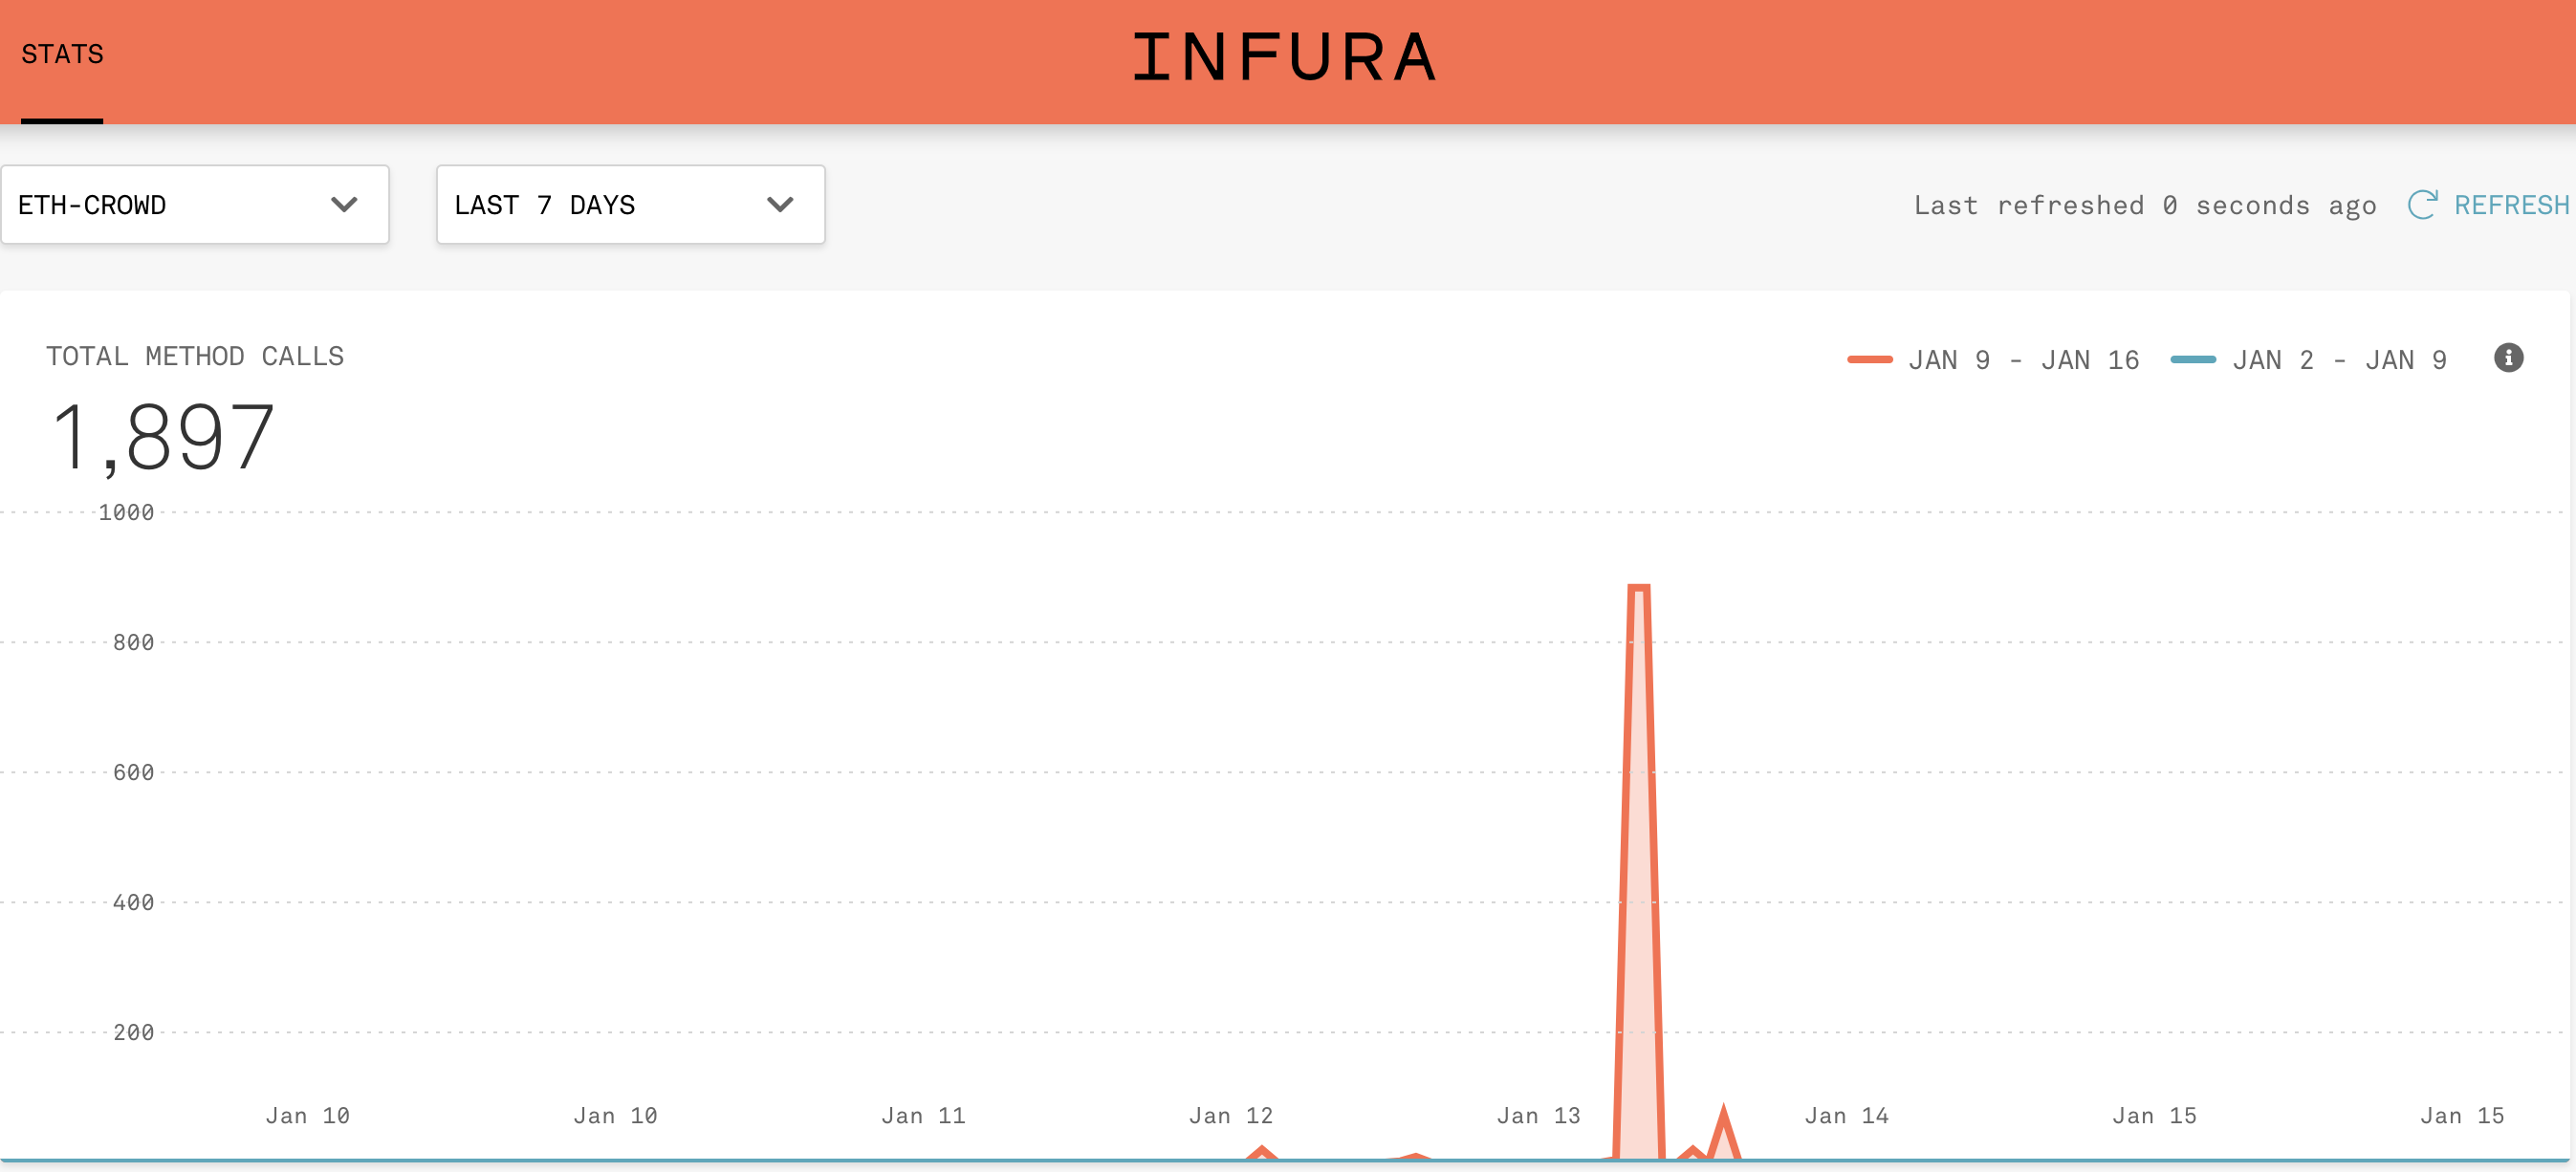
\includegraphics[width=0.8\textwidth]{infura-calls-3}
\caption[infuracalls3]{En el gráfico se ve el pico de actividad en la API cuando estaba sucediendo el bug del loop infinito.}
\label{fig:infura-calls-3}
\end{figure}


\subsection{Semana 8}
Durante esta semana se terminaron de escribir las primeras versiones de los capítulos 1 y 2
del informe y a su vez se comenzó a escribir el capítulo 3. Además, se hicieron diversas pruebas 
que llevaron más de 15 horas combinando versiones de Node, solc, web3, pragma solidity y del
compilador solidity para dar con la combinación definitiva para llevar adelante la app (28).

Las versiones finales que se encontraron 100\% compatibles y estables y que serán utilizadas para
todo el proyecto son:

\begin{itemize}
	\item Node v8.11.4
	\item Pragma Solidity \^0.4.17;
	\item Compiler (solo en Remix) 0.4.19+commit.c4cbbb05.Emscripten.clang
	\item Solc 0.4.19
	\item Web3 1.0.0-beta.26
\end{itemize}

\begin{figure}[htbp!] 
\centering    
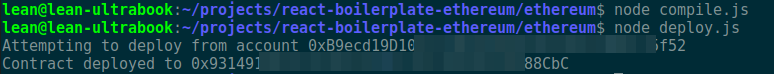
\includegraphics[width=0.9\textwidth]{success-deploy}
\caption[successdeploy]{Comandos para compilar y deployar funcionando correctamente. Se puede ver que cuando el contrato es deployado, se nos devuelve la dirección donde ha sido deployado.}
\label{fig:success-deploy}
\end{figure}

\subsection{Semana 9}
Teniendo seleccionadas las versiones estables del ecosistema de la app, se procedió a escribir
el código encargado de consumir los métodos de los contratos Project y ProjectBuilder (34).
Se escribió el código para conectarse a los contratos a través de web3 (35). Se probaron con éxito
las dos tareas previas.

Se hizo el set up completo del entorno front end con React, React Router, Webpack y Babel (36).

Se hicieron retoques en los capítulos 1 y 2 del informe y se continuó trabajando sobre el capítulo
3.

Se hizo el componente Index en React, el cual a través de web3 obtiene y muestra todos los
proyectos creados en la dirección que se le haya configurado (37).

\subsection{Semana 10}
Esta semana fue intensa en cuanto a desarrollo del front end, se investigó sobre buenas prácticas
en React y se pudieron hacer los componentes correspondientes a los tickets 39, 40, 41, 42, 43
y 44 (únicamente el HTML y Javascript, restando para la semana siguiente el CSS). En este punto
ya se puede decir que tenemos una aplicación completamente funcional, todos los componentes del 
front end desencadenan las acciones correspondientes para conectarse con los contratos y recibir
o enviar información. También el back end se encuentra completamente funcional, todos los comandos
creados funcionan correctamente. 

Se hicieron más retoques en los capítulos 1 y 2, también se añadieron imágenes.

Resta agregar los estilos a los componentes.

\subsection{Semana 11}
Durante esta semana se agregaron los estilos CSS a la aplicación, específicamente a los componentes
relacionados a los tickets 39, 40, 41, 42, 43 y 44. 

Se actualizó el capítulo 3 del informe hasta la semana 11 inclusive.


\subsection{Semana 12}
Esta semana se trabajó fuertemente en el capítulo 4 y 5 del informe, exponiendo los resultados de la aplicación desarrollada. Así mismo se fixearon algunos bugs mínimos mayormente de estilos en la 
aplicación.

Se cerró el capítulo 5 con la conclusión y con posibilidades de continuar el trabajo tomando este
informe como punto de partida.

Se hizo y completó la sección de \textit{Referencias}.

Con todo esto, queda concluída la primer versión final del informe lista para ser entregada.

%%!TEX root = ../thesis.tex
%*******************************************************************************
%****************************** Fourth Chapter *********************************
%*******************************************************************************

\chapter{Marco teórico}

\ifpdf
    \graphicspath{{Chapter4/Figs/}{Chapter4/Figs/PDF/}{Chapter4/Figs/}}
\else
    \graphicspath{{Chapter4/Figs/}{Chapter4/Figs/}}
\fi


\section{Resultados}

\subsection{}


%%!TEX root = ../thesis.tex
%*******************************************************************************
%****************************** Fifth Chapter *********************************
%*******************************************************************************

\chapter{Conclusión}

\ifpdf
    \graphicspath{{Chapter5/Figs/}{Chapter5/Figs/PDF/}{Chapter5/Figs/}}
\else
    \graphicspath{{Chapter5/Figs/}{Chapter5/Figs/}}
\fi


\section{Resultados}
Se completó el desarrollo en un tiempo aceptable y cumpliendo los objetivos personales propuestos
tanto en la aplicación desarrollada como en el presente informe. Se incorporaron nuevas tecnologías
como blockchain, Ethereum y Solidity. También se profundizaron otras como Node y React, esta última
particularmente.

Gracias al hincapié de estudiar e investigar las nuevas tecnologías elegidas para el proyecto, se
comenzó a trabajar en el código con una cierta confianza conociendo de manera sólida todos los
procesos que estaban pasando detrás de la implementación del código.

Considero un éxito el presente desarrollo debido a la gran cantidad de nuevo conocimiento
incorporado en tecnologías que se encuentran en auge y por el hecho de haberlo plasmado en una app
100\% funcional.


\subsection{Posibilidades con este informe como punto de partida}
En la presente sección se enumerarán algunas opciones viables en caso de que alguien decida tomar
como punto de partida este informe para su tesina. Un punto importante es que destaco que las
opciones presentadas son altamente recomendadas para los alumnos que no posean experiencia laboral 
o que recién hayan comenzado su carrera profesional.

\begin{itemize}
	\item Actualizar Node y todas las dependencias utilizadas a su última versión estable. Esto
	obligará también a actualizar el código del contrato Solidity y los scripts de compilación y
	deploy. Actualizar dependencias y código acorde es una práctica común en el ámbito laboral real
	y muchas veces resulta ser excesivamente complejo llevarlo a cabo por todas las consideraciones
	que	se deben tener en cuenta respecto al código en producción. 
	
	\item Desarrollar dentro de la app proyectada un sistema de usuarios, donde para acceder a la
	app el usuario deba registrarse y loguearse (en favor de esto y de las prácticas comunes en el
	mercado laboral será agregar social login). A cada usuario le serán añadidas sus wallets y al
	momento de transaccionar se deberá asegurar que el wallet logueado en Metamask coincida con
	alguno de los adjuntos al usuario. A su vez, relacionar también los proyectos con los usuarios,
	donde los proyectos tendrán un usuario como owner/responsable (al igual que el contrato ahora
	mismo) y los usuarios tendrán un registro de los proyectos que participan como backers y los
	payments que aprueban o desaprueban. Queda a elección si usar una base de datos SQL o NoSQL.
	
	\item Investigar y desarrollar desde el punto de vista de la inversión en criptomonedas debido
	a que en el presente informe se ha indicado que no se hablaría en absoluto sobre inversiones.

\end{itemize}

%\include{Chapter6/chapter6}
%\include{Chapter7/chapter7}



% ********************************** Back Matter *******************************
% Backmatter should be commented out, if you are using appendices after References
%\backmatter

% ********************************** Bibliography ******************************
\begin{spacing}{0.9}

% To use the conventional natbib style referencing
% Bibliography style previews: http://nodonn.tipido.net/bibstyle.php
% Reference styles: http://sites.stat.psu.edu/~surajit/present/bib.htm

\bibliographystyle{apalike}
%\bibliographystyle{unsrt} % Use for unsorted references  
%\bibliographystyle{plainnat} % use this to have URLs listed in References
\cleardoublepage
\bibliography{References/references} % Path to your References.bib file


% If you would like to use BibLaTeX for your references, pass `custombib' as
% an option in the document class. The location of 'reference.bib' should be
% specified in the preamble.tex file in the custombib section.
% Comment out the lines related to natbib above and uncomment the following line.

%\printbibliography[heading=bibintoc, title={References}]


\end{spacing}

% ********************************** Appendices ********************************

\begin{appendices} % Using appendices environment for more functunality

%%!TEX root = ../thesis.tex
% ******************************* Thesis Appendix A ****************************
\chapter{How to install \LaTeX} 

\section*{Windows OS}

\subsection*{TeXLive package - full version}
\begin{enumerate}
\item	Download the TeXLive ISO (2.2GB) from\\
\href{https://www.tug.org/texlive/}{https://www.tug.org/texlive/}
\item	Download WinCDEmu (if you don't have a virtual drive) from \\
\href{http://wincdemu.sysprogs.org/download/}
{http://wincdemu.sysprogs.org/download/}
\item	To install Windows CD Emulator follow the instructions at\\
\href{http://wincdemu.sysprogs.org/tutorials/install/}
{http://wincdemu.sysprogs.org/tutorials/install/}
\item	Right click the iso and mount it using the WinCDEmu as shown in \\
\href{http://wincdemu.sysprogs.org/tutorials/mount/}{
http://wincdemu.sysprogs.org/tutorials/mount/}
\item	Open your virtual drive and run setup.pl
\end{enumerate}

or

\subsection*{Basic MikTeX - \TeX~ distribution}
\begin{enumerate}
\item	Download Basic-MiK\TeX (32bit or 64bit) from\\
\href{http://miktex.org/download}{http://miktex.org/download}
\item	Run the installer 
\item	To add a new package go to Start >> All Programs >> MikTex >> Maintenance (Admin) and choose Package Manager
\item	Select or search for packages to install
\end{enumerate}

\subsection*{TexStudio - \TeX~ editor}
\begin{enumerate}
\item	Download TexStudio from\\
\href{http://texstudio.sourceforge.net/\#downloads}
{http://texstudio.sourceforge.net/\#downloads} 
\item	Run the installer
\end{enumerate}

\section*{Mac OS X}
\subsection*{MacTeX - \TeX~ distribution}
\begin{enumerate}
\item	Download the file from\\
\href{https://www.tug.org/mactex/}{https://www.tug.org/mactex/}
\item	Extract and double click to run the installer. It does the entire configuration, sit back and relax.
\end{enumerate}

\subsection*{TexStudio - \TeX~ editor}
\begin{enumerate}
\item	Download TexStudio from\\
\href{http://texstudio.sourceforge.net/\#downloads}
{http://texstudio.sourceforge.net/\#downloads} 
\item	Extract and Start
\end{enumerate}


\section*{Unix/Linux}
\subsection*{TeXLive - \TeX~ distribution}
\subsubsection*{Getting the distribution:}
\begin{enumerate}
\item	TexLive can be downloaded from\\
\href{http://www.tug.org/texlive/acquire-netinstall.html}
{http://www.tug.org/texlive/acquire-netinstall.html}.
\item	TexLive is provided by most operating system you can use (rpm,apt-get or yum) to get TexLive distributions
\end{enumerate}

\subsubsection*{Installation}
\begin{enumerate}
\item	Mount the ISO file in the mnt directory
\begin{verbatim}
mount -t iso9660 -o ro,loop,noauto /your/texlive####.iso /mnt
\end{verbatim}

\item	Install wget on your OS (use rpm, apt-get or yum install)
\item	Run the installer script install-tl.
\begin{verbatim}
	cd /your/download/directory
	./install-tl
\end{verbatim}
\item	Enter command `i' for installation

\item	Post-Installation configuration:\\
\href{http://www.tug.org/texlive/doc/texlive-en/texlive-en.html\#x1-320003.4.1}
{http://www.tug.org/texlive/doc/texlive-en/texlive-en.html\#x1-320003.4.1} 
\item	Set the path for the directory of TexLive binaries in your .bashrc file
\end{enumerate}

\subsubsection*{For 32bit OS}
For Bourne-compatible shells such as bash, and using Intel x86 GNU/Linux and a default directory setup as an example, the file to edit might be \begin{verbatim}
edit $~/.bashrc file and add following lines
PATH=/usr/local/texlive/2011/bin/i386-linux:$PATH; 
export PATH 
MANPATH=/usr/local/texlive/2011/texmf/doc/man:$MANPATH;
export MANPATH 
INFOPATH=/usr/local/texlive/2011/texmf/doc/info:$INFOPATH;
export INFOPATH
\end{verbatim}
\subsubsection*{For 64bit OS}
\begin{verbatim}
edit $~/.bashrc file and add following lines
PATH=/usr/local/texlive/2011/bin/x86_64-linux:$PATH;
export PATH 
MANPATH=/usr/local/texlive/2011/texmf/doc/man:$MANPATH;
export MANPATH 
INFOPATH=/usr/local/texlive/2011/texmf/doc/info:$INFOPATH;
export INFOPATH

\end{verbatim}



%\subsection{Installing directly using Linux packages} 
\subsubsection*{Fedora/RedHat/CentOS:}
\begin{verbatim} 
sudo yum install texlive 
sudo yum install psutils 
\end{verbatim}


\subsubsection*{SUSE:}
\begin{verbatim}
sudo zypper install texlive
\end{verbatim}


\subsubsection*{Debian/Ubuntu:}
\begin{verbatim} 
sudo apt-get install texlive texlive-latex-extra 
sudo apt-get install psutils
\end{verbatim}

%%!TEX root = ../thesis.tex
% ******************************* Thesis Appendix B ********************************

\chapter{Installing the CUED class file}

\LaTeX.cls files can be accessed system-wide when they are placed in the
<texmf>/tex/latex directory, where <texmf> is the root directory of the user’s \TeX installation. On systems that have a local texmf tree (<texmflocal>), which
may be named ``texmf-local'' or ``localtexmf'', it may be advisable to install packages in <texmflocal>, rather than <texmf> as the contents of the former, unlike that of the latter, are preserved after the \LaTeX system is reinstalled and/or upgraded.

It is recommended that the user create a subdirectory <texmf>/tex/latex/CUED for all CUED related \LaTeX class and package files. On some \LaTeX systems, the directory look-up tables will need to be refreshed after making additions or deletions to the system files. For \TeX Live systems this is accomplished via executing ``texhash'' as root. MIK\TeX users can run ``initexmf -u'' to accomplish the same thing.

Users not willing or able to install the files system-wide can install them in their personal directories, but will then have to provide the path (full or relative) in addition to the filename when referring to them in \LaTeX.

\end{appendices}

% *************************************** Index ********************************
\printthesisindex % If index is present

\end{document}
